\documentclass[titlepage, 12pt]{article}
\usepackage[utf8]{inputenc}
\usepackage[spanish]{babel}
\usepackage{fancyhdr}
\usepackage{graphicx}
\usepackage{geometry}
\usepackage{setspace}
\usepackage{float}
\usepackage{titlesec}
\usepackage{titling}
\usepackage{amsmath}
\usepackage{amsfonts}
\onehalfspacing


\title{\textbf{Docking molecular de la proteína E del SARS-CoV-2 y la amantadina}}

\author{
    M. en NE. Rodrigo Ramírez Rodríguez \\
                Doctorado en Investigaciones Cerebrales\\
        Instituto de Investigaciones Cerebrales\\
        Xalapa, México
            }
\date{\today}

\begin{document}

\maketitle

\begin{abstract}
El virus del SARS-CoV-2 a comprometido la salud a nivel mundial. A pesar de la amplia investigación sobre este virus sólo han emergido propuestas farmacológicas no testadas contra este virus. La proteína E de este virus es la responsable de establecer viroporinas y diseminar el virus en el hospedero. La amantadina es un antiviral que pudiera tener una actividad potencial contra la proteína E. El objetivo de este estudio reside en hacer un modelaje de la interacción ligando-proteína a través de docking para determinar cualés son los sitios con los que el fármaco interacciona con el virus. Se obtuvieron las estructuras moleculares de la amantadina (DB00915) y de la proteína E (7K3G) de respectivos bancos y fueron sometidos a un proceso de docking molecular en Autodock y Autodock Vina. Los resultados indican que la amantadina interacciona en los aminoácidos Leucina 18 y Asparagina 15 de la proteína E. Dichos aminoácidos son parte del dominio de transmembrana hidrofóbica los cuales facilitan la formación de viroporinas, por lo tanto, la amantadina es un potencial fármaco antiviral contra la proteína E del SARS-CoV-2.
\end{abstract}


\section{Introducción}

El virus del SARS-CoV-2 ha afectado la salud en humanos principalmente en vías respiratorias, en particular, produciendo neumonia y eventualmente una falla respiratoria aguda (Mohanty et al., 2020). A nivel del sistema nervioso central, se reporta que las acciones de este virus ocurren en la amígdala, la corteza cerebral y el tallo cerebral (pons y medula oblongata), cuyas regiones cerebrales son críticas en los procesos respiratorios (Lukiw et al., 2020).

Para controlar las sintomatologías del virus, se han optado por la implementación de fármacos que están asociados a mecanismos conocidos de otros virus como es la inhibición de síntesis de proteínas (Lai et al., 2020, Zheng, 2020). Sin embargo, estas medidas no han sido experimental probadas en el virus del SARS-CoV-2 por lo que los mecanismos de dichos fármacos y sus acciones en este virus son hipotéticas.

El SARS-CoV-2 tiene tres proteínas principales que actúan para ingresar hacia su hospedero: la proteína Spike, la proteína de membrana y la proteína E. De estas, la proteína envelope o E actúa liberando viriones que se ensamblan en la membrana celular del hospedero formando viroporinas las cuales son proteínas que modifican la membrana celular formando poros de caracter proteína-lípido que están involucrados en el transporte de iones, por lo que se ha convertido en un epicentro de intervención farmacólogica (Naqvi et al., 2020).

La estructura de la proteína E posee una región hidrofóbica la cual se denomina como el dominio de transmembrana hidrofóbica la cual contiene una alfa hélice que se oligomeriza para formar los poros en las membranas (Schoeman y Fielding, 2020). Se reporta que la mutación en algunos aminoácidos como la asparagina 15 y valina 25 del dominio de transmembrana hidrofóbica produce una falla en la formación de las viroporinas (Schoeman y Fielding, 2020). Por tanto, la afección en los aminoácidos en este dominio es clave en la intervención farmacológica.

A través de los modelos in silico se ha logrado modelar la interacción de la estructura de la proteína E con potenciales fármacos como fitoquímicos (Gupta et al., 2020). Sin embargo, se necesita el uso de fármacos estandarizados y de fácil acceso económico y de receta médica disponible para la población. Un estudio reciente muestra que el docking de la proteína E con la amantadina, un antiviral implicado en la ruptura de puentes de hidrógenos que eventualmente previene la entrada del virion, muestra que dicho antiviral interactúa con los puentes de hidrógeno de los aminoácidos alanina 22 y fenilalanina 26, este último forma parte de la alfa hélice del dominio de transmembrana (Aranda-Abreu et al., 2020). 


\section{Descripción del problema a resolver}

Dado que el modelo de la proteína E contiene diversos modelos, esta investigación tuvo como objetivo realizar el Docking de un modelo estructural de la proteína E usando como ligando a la amantadina. La proteína E (7K3G) se adquirió de Protein Data Bank y la amantadina (DB00915) se adquirió de DrugBank Online. Mediante Autodock y Autodock Vina se determinaron cualés son los aminoácidos con los que la amantadina interacciona con el dominio de transmembrana hidrofóbico de la proteína E y la respectiva energía de afinidad. 

\section{Resultados}

Del docking, con la semilla aleatoria -834651280, se obtuvieron nueve conformaciones del ligando DB00915 
(Figura \ref{docking}). El modo 1 indica una alta energía de afinidad de -5.5 (kcal/mol)(Figura \ref{modo 1}). 


\begin{figure}
    \centering
    \includegraphics[width=0.5\textwidth]{Dockeo.png}
    \caption{Conformaciones de DB00915 con la proteína E del SARS-Cov-2}
    \label{docking}
\end{figure}


\begin{figure}
    \centering
    \includegraphics[width=0.5\textwidth]{conformación 1.png}
    \caption{Conformación 1 de DB00915 con la proteína E del SARS-CoV-2}
    \label{modo 1}
\end{figure}


Los resultados de Vina indican que el DB00915 interacciona con la proteína E mediante la unión con puentes de hidrógenos de los aminoácidos Leucina 18 y Asparagina 15.

\begin{figure}
    \centering
    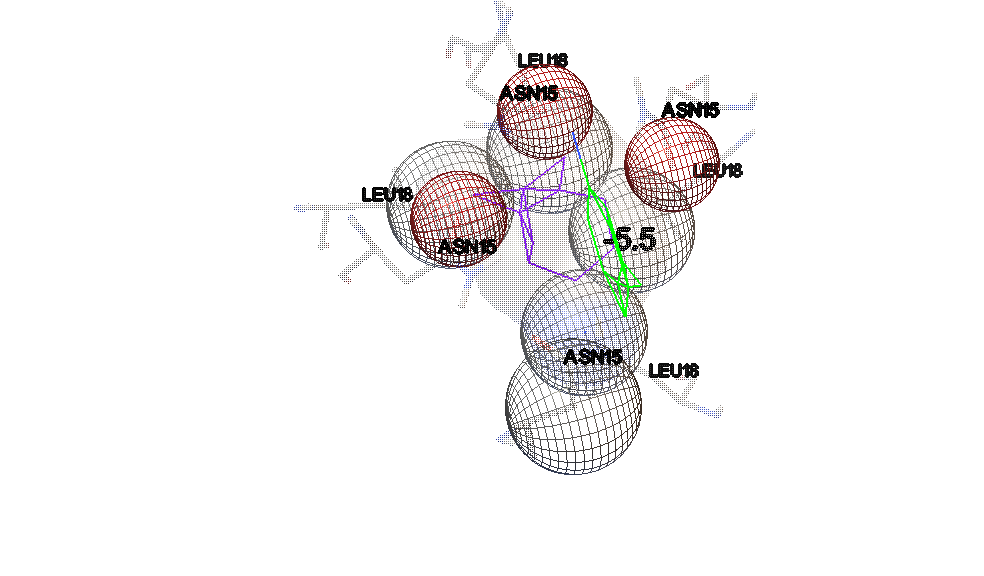
\includegraphics[width=1\textwidth]{Docking Protein E - amantadina.png}
    \caption{Interacción de los aminoácidos LEU 18 y ASN 15 en la conformación 1 de DB00915 con la proteína E del SARS-CoV-2}
    \label{aminoácidos}
\end{figure}

\section{Conclusiones}

La amantadina ha mostrado tener sitios de unión en la proteína SARS-CoV-2 en alanina 22 y fenilalanina 26 (Aranda-Abreu et al., 2020). Los resultados de este experimento por Docking indican que la amantadina tiene otros sitios de unión en los aminoácidos LEU 18 y ASN 15. Esto sugiere que la amantadina puede actuar en diversos puntos de unión de esta proteína E reduciendo la capacidad del dominio de transmembrana hidrofóbico para forma viroporinas. Estos datos apoyan el uso de la amantadina como un potencial fármaco para mitigar los efectos del SARS-CoV-2.


\section{Referencias}


Aranda-Abreu, G. E., Hernández-Aguilar, M. E., Herrera-Covarrubias, D. y Rojas-Durán, F. (2020). Amantadine as a drug to mitigate the effects of COVID-19. Medical Hypothesis. https://doi.org/10.1016/j.mehy.2020.109755

Gupta, M. K., Vemula, S., Donde, R., Gouda, G., Behera, L. y Vadde, R. (2020). In-silico aprroaches to detect inhibitors of the human severe acute respiratory syndrome coronavirus envelope protein ion channel. Journal of Biomolecular Structure and Dynamics. https://doi.org/10.1080/07391102.2020.1751300

Lai,C-C., Shih, T-P., Ko, W-C., Tang, H-J. y Hsueh, P-R. (2020). 
Severe acute respiratory syndrome coronavirus 2 (SARS-CoV-2) and coronavirus disease-2019 (COVID-19): the epidemic and the challenges. 
International Journal of Antimicrobial Agents.
https://doi.org/10.10162Fj.ijantimicag.2020.105924

Lukiw, W. J., Pogue, A. y Hill, J. M. (2020). SARS-CoV-2 infectivity and neurological targets in the brain. Cellular and Molecular Neurobiology, 25, 1-8.

Mohanty, S. K., Satapathy, A., Naidu, M. M., Mukhopadhyay, S., Sharma, S., Barton, L. M., Stroberg, E., Duval, E. J., Pradhan, D., Tzankov, A. y Parwani, A. V. (2020). Severe acute respiratory syndrome coronavirus-2 (SARS-CoV-2) and coronavirus disease 19 (COVID-19) - anatomic pathology perspective on current knowledge. Diagnostic Pathology.
https://doi.org/10.11862Fs13000-020-01017-8

Naqvi, A. A. T., Fatima, K., Mohammad, T., Fatima, U., Singh, I. K., Singh, A., Atif, S. M., Hariprasad, G., Hasan, G. M. y Hassan, M. I. (2020). Insights into SARS-CoV-2 genome, structure, evolution, pathogenesis and therapies: structural genomics approach. Biochimica et Biophsyca Acta Molecular Basis of Disease. https://doi.org/10.1016/j.bbadis.2020.165878

Shoeman, D. y Fielding, B. C. (2020). Coronavirus envelope protein: current knowledge. Virology Journal. https://doi.org/10.1186/s12985-019-1182-0

Zheng, J. (2020). SARS-CoV-2: an emerging coronavirus that causes a global threat. International Journal of Biological Sciences. 16, 1678-1685.

\end{document}

